\documentclass[aspectratio=169, table, 12pt]{beamer}

\usepackage{colortbl}
\usepackage{xcolor}
\usepackage{listings}
\usepackage{tabularx}
\usepackage{tikz}
\usetikzlibrary{arrows.meta, positioning, calc, fit,
  shapes.geometric, backgrounds}

\makeatletter
\def\input@path{{../theme/}}
\makeatother
\graphicspath{{../theme/}{../../figures/}}
\usetheme{Pradita}

\definecolor{praditagreen}{RGB}{37, 113, 71}

% Tema membuat garis tabel berwarna putih. Dikembalikan agar tabel terbaca.
\arrayrulecolor{black}
\setlength{\arrayrulewidth}{0.5pt}

\lstdefinestyle{PythonStyle}{
  language=Python,
  basicstyle=\ttfamily\scriptsize,
  keywordstyle=\color{blue}\bfseries,
  commentstyle=\color{gray}\itshape,
  stringstyle=\color{red},
  breaklines=true,
  frame=lines,
  backgroundcolor=\color{lightgray!10},
  tabsize=2,
  showstringspaces=false
}

\lstdefinelanguage{bash}{
  keywords={},
  basicstyle=\ttfamily\scriptsize,
  ndkeywords={cd, python, bash, source},
  ndkeywordstyle=\color{purple}\bfseries,
  sensitive=true,
  commentstyle=\color{gray},
  breaklines=true,
  frame=lines,
  backgroundcolor=\color{lightgray!10},
  tabsize=2,
  comment=[l]{\#},
  showstringspaces=false
}

\title{\Huge{Serverless Architecture}}
\subtitle{IF231303 Arsitektur Perangkat Lunak}
\author{Alfa Yohannis}

\begin{document}

\frame{\titlepage}

\begin{frame}{{\Large Tujuan Pembelajaran}}
  \vspace{10pt}
  \begin{enumerate}
    \item Menjelaskan pembagian antara fungsi, event, dan penjalan beserta
          kontrak yang menghubungkan ketiganya.
    \item Membedakan \textit{cold start} dari \textit{warm start}, lalu
          menentukan kapan susunan tanpa server layak dipilih.
    \item Mengukur \textit{cold start cost}, \textit{idle cost}, dan
          \textit{concurrency limit} pada penjalan fungsi dibanding layanan
          yang hidup terus.
  \end{enumerate}

  \vspace{10pt}
  {\small Contohnya tiga fungsi kecil, yaitu konversi kurs, pemeriksaan
  pesanan, dan penghitungan pajak.}
\end{frame}

\begin{frame}{{\Large Pendahuluan}}
  \vspace{8pt}
  \begin{itemize}\small
    \item Bab sebelumnya memakai satu anggapan yang sama, yaitu ada proses yang
          hidup terus menunggu \textit{request}.
    \item Anggapan itu menjadi mahal ketika \textit{request}-nya jarang, sebab proses
          yang menganggur tetap memegang memori dan tetap ditagih.
    \item \textit{Serverless} membalik anggapan itu, yaitu kode dimuat ketika
          ada kabar yang menuntutnya, lalu dilepas kembali.
    \item Satuan penyebarannya satu fungsi, dan bentuk itu disebut
          Function-as-a-Service (FaaS).
  \end{itemize}

  \vspace{8pt}
  {\small Namanya menyesatkan, sebab servernya tetap ada. Yang hilang adalah
  urusan menyediakan dan menjaga server itu.}
\end{frame}

\begin{frame}{{\Large Istilah yang Dipakai}}
  \vspace{10pt}
  \begin{itemize}\small
    \item \textbf{Fungsi} adalah satu kemampuan kecil yang menjawab satu jenis
          kabar.
    \item \textbf{Event} adalah kabar yang datang beserta muatannya.
    \item \textbf{Penjalan} adalah pihak yang memuat fungsi, memanggilnya, lalu
          melepasnya kembali.
    \item \textbf{Manifes} adalah \textit{file} JSON berisi nama event, nama modul,
          nama kelas, dan besar memori yang dipesan.
  \end{itemize}

  \vspace{10pt}
  {\small Penjalan tidak mengenal satu nama fungsi pun. Yang dikenalnya hanya
  bentuk kontrak beserta registri manifes.}
\end{frame}

\begin{frame}{{\Large Alur Satu Event}}
  \vspace{6pt}
  \begin{center}
    \resizebox{0.82\textwidth}{!}{%
      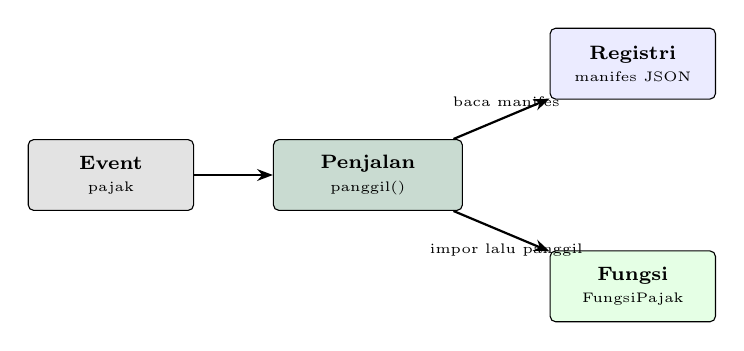
\begin{tikzpicture}[
        kotak/.style={draw, rounded corners=2pt, minimum width=2.1cm,
          minimum height=0.9cm, align=center, font=\scriptsize\bfseries},
        panah/.style={-{Stealth[length=2mm]}, thick}
      ]
        \node[kotak, fill=gray!22] (event) {Event\\
          {\tiny\mdseries pajak}};
        \node[kotak, fill=praditagreen!25, right=1.0cm of event,
          minimum width=2.4cm] (penjalan) {Penjalan\\
          {\tiny\mdseries panggil()}};
        \node[kotak, fill=blue!8, above right=0.5cm and 1.1cm of penjalan]
          (registri) {Registri\\{\tiny\mdseries manifes JSON}};
        \node[kotak, fill=green!10, below right=0.5cm and 1.1cm of penjalan]
          (fungsi) {Fungsi\\{\tiny\mdseries FungsiPajak}};

        \draw[panah] (event) -- (penjalan);
        \draw[panah] (penjalan) -- node[above, font=\tiny, pos=0.55]
          {baca manifes} (registri);
        \draw[panah] (penjalan) -- node[below, font=\tiny, pos=0.55]
          {impor lalu panggil} (fungsi);
      \end{tikzpicture}}
  \end{center}

  \vspace{4pt}
  {\small Nama kelas fungsinya tertulis di manifes, bukan di dalam kode
  penjalan. Manifes dibaca tanpa mengimpor satu baris kode fungsi pun.}
\end{frame}

\begin{frame}{{\Large Tanggung Jawab Ketiga Peran}}
  \vspace{6pt}
  \centering
  \small
  \begin{tabularx}{0.96\textwidth}{|l|X|X|}
    \hline
    \textbf{Peran} & \textbf{Tanggung jawab} & \textbf{Tidak boleh mengetahui} \\
    \hline
    Fungsi & Menyiapkan bahannya di konstruktor lalu melayani satu event & Siapa yang memanggilnya dan berapa lama contohnya disimpan \\
    \hline
    Penjalan & Memuat modul, memanggil penangan, lalu melepas contoh yang diam & Nama kelas mana pun, sebab namanya dibaca dari manifes \\
    \hline
    Registri & Membaca seluruh manifes lalu menjawab pertanyaan tentang event & Isi kode fungsinya, sebab manifes dibaca tanpa mengimpor \\
    \hline
  \end{tabularx}

  \vspace{6pt}
  \raggedright
  {\small Fungsi tidak tahu berapa lama contohnya disimpan, padahal penyimpanan
  itulah yang menentukan mahal atau murahnya pemanggilan berikutnya.}
\end{frame}

\begin{frame}[fragile]{{\Large Kode: Kontrak Fungsi}}
  \vspace{4pt}
\begin{lstlisting}[style=PythonStyle]
class Fungsi(Protocol):
  """Satu kemampuan kecil yang dimuat penjalan ketika event-nya datang."""

  def __init__(self) -> None:
    """Menyiapkan seluruh bahan yang dipakai berulang oleh penangan."""

  def tangani(self, event: dict) -> dict:
    """Melayani satu event lalu mengembalikan dict berisi hasilnya."""
\end{lstlisting}

  \vspace{4pt}
  {\small Kontraknya sempit, yaitu konstruktor tanpa argumen ditambah satu
  metode penangan. Pembagian itulah yang menentukan letak biaya.}
\end{frame}

\begin{frame}{{\Large Tiga Fase Daur Hidup}}
  \vspace{10pt}
  \begin{itemize}\small
    \item \texttt{Init} memuat modulnya lalu membuat objeknya. Seluruh
          persiapan berat dibayar di sini.
    \item \texttt{Invoke} memanggil penangan dengan muatan \textit{event}-nya.
    \item \texttt{Shutdown} melepas objek yang sudah lama diam, dan modulnya
          dikeluarkan dari \textit{import cache} Python.
    \item Ketiga namanya diambil dari dokumentasi AWS Lambda, dan urutannya
          sama persis.
  \end{itemize}

  \vspace{10pt}
  {\small Tanpa langkah mengeluarkan modul dari cache, pemanggilan berikutnya
  hanya membaca cache, sehingga \textit{cold start} terlihat jauh lebih murah
  daripada yang sebenarnya.}
\end{frame}

\begin{frame}[fragile]{{\Large Kode: Init dan Shutdown}}
  \vspace{2pt}
\begin{lstlisting}[style=PythonStyle]
def bangun_objek(self, event: str):
  """Mengimpor modul fungsinya lalu membuat objeknya, yaitu fase Init."""
  manifes = self.pendaftar.manifes_untuk(event)
  modul = importlib.import_module(manifes["modul"])
  kelas = getattr(modul, manifes["kelas"])
  return kelas()
def lupakan_modul(self, event: str) -> None:
  """Mengeluarkan modul fungsinya dari cache impor Python."""
  nama = self.pendaftar.manifes_untuk(event)["modul"]
  sys.modules.pop(nama, None)
  nama_paket, _, nama_anak = nama.rpartition(".")
  paket = sys.modules.get(nama_paket)
  if paket is not None and hasattr(paket, nama_anak):
    delattr(paket, nama_anak)
\end{lstlisting}

  \vspace{2pt}
  {\small Fungsi kedua dipanggil ketika contoh terakhir dilepas, dan itulah
  yang membuat \textit{scale to zero}, atau turun ke nol, terjadi.}
\end{frame}

\begin{frame}{{\Large \textit{Sequence Diagram}: \textit{Cold} dan \textit{Warm}}}
  \vspace{4pt}
  \begin{center}
    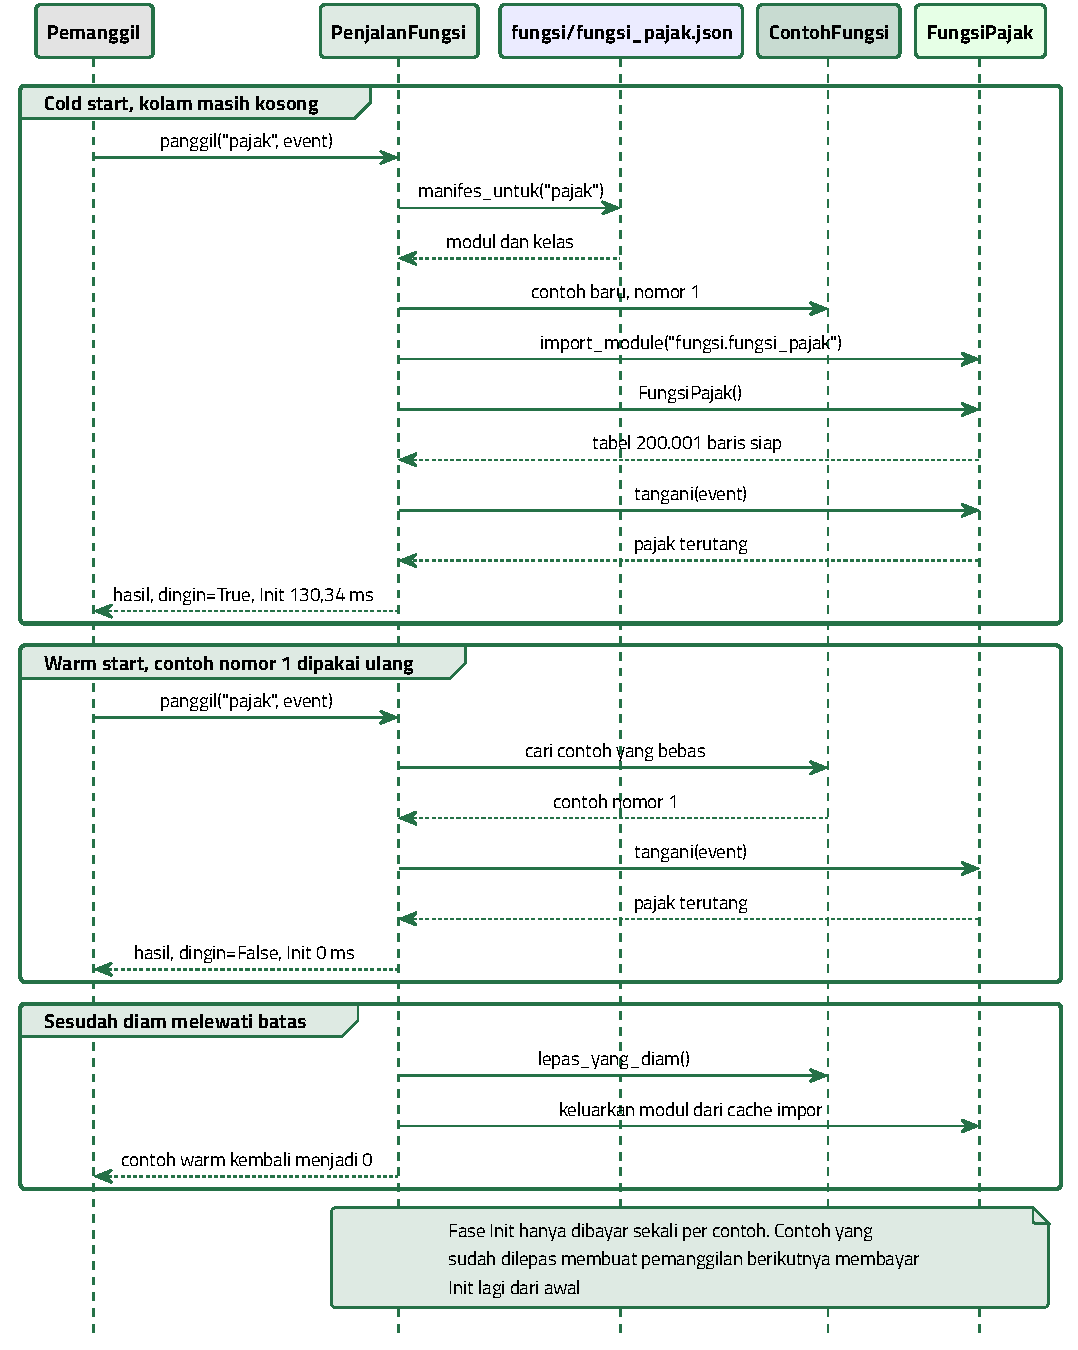
\includegraphics[width=0.92\textwidth, height=0.74\textheight,
      keepaspectratio]{sekuens-serverless.pdf}
  \end{center}
\end{frame}

\begin{frame}{{\Large Penjelasan \textit{Sequence Diagram}}}
  \vspace{10pt}
  \begin{itemize}\small
    \item \textit{Cold start} menempuh impor beserta pembuatan objek lebih
          dahulu, lalu baru masuk fase \texttt{Invoke}.
    \item \textit{Warm start} menemukan contoh siap pakai, sehingga langsung
          masuk fase \texttt{Invoke}.
    \item Pekerjaan domainnya sama persis pada keduanya, yang berbeda siapa
          yang membayar fase \texttt{Init}.
    \item Sesudah contohnya diam melewati batas, contohnya dilepas dan keadaan
          kembali ke nol.
  \end{itemize}

  \vspace{10pt}
  {\small Menjalankan \texttt{python penjalan.py} memperlihatkan ketiganya
  berurutan, yaitu \texttt{Init} 130,342 ms, lalu nol, lalu \texttt{Init} lagi
  sesudah didiamkan 2,2 detik.}
\end{frame}

\begin{frame}{{\Large Analogi: Lampu Koridor}}
  \vspace{10pt}
  \begin{itemize}\small
    \item Koridor yang kosong gelap total dan tidak menghabiskan daya sedikit
          pun.
    \item Orang pertama yang lewat menunggu sesaat sampai lampunya terang
          penuh.
    \item Orang berikutnya tidak menunggu apa pun, sebab lampunya masih
          menyala.
    \item Beberapa menit sesudah koridornya sepi, lampu itu padam kembali
          dengan sendirinya.
  \end{itemize}

  \vspace{10pt}
  {\small Menunggu sesaat itulah \textit{cold start}, menyala terus itulah
  \textit{warm start}, dan padam sendiri itulah \textit{scale to zero}.}
\end{frame}

\begin{frame}{{\Large Hasil: \textit{Cold Start Cost}}}
  \vspace{6pt}
  {\small Dua ratus panggilan per fungsi, setiap panggilan kelima sengaja
  dibuat menjadi \textit{cold start}. Satuannya milidetik.}

  \vspace{6pt}
  \centering
  \small
  \begin{tabularx}{0.96\textwidth}{|X|l|l|}
    \hline
    \textbf{Yang diukur} & \textbf{Fungsi kurs} & \textbf{Fungsi pajak} \\
    \hline
    Median \textit{cold start} & 0,2414 & 120,5837 \\
    \hline
    Terbesar \textit{cold start} & 0,9045 & 129,0490 \\
    \hline
    Median \textit{warm start} & 0,0027 & 0,0059 \\
    \hline
    Terbesar \textit{warm start} & 0,0379 & 0,0536 \\
    \hline
    \textit{Cold start} lebih lambat & 90,4 kali & 20.554,8 kali \\
    \hline
  \end{tabularx}
\end{frame}

\begin{frame}{{\Large Membaca Hasilnya}}
  \vspace{10pt}
  \begin{itemize}\small
    \item Median \textit{warm start} kedua fungsi, 0,0027 dan 0,0059 ms, belum
          dapat dibedakan, padahal persiapannya jauh berbeda.
    \item Sebabnya persiapan berat sudah dibayar pada fase \texttt{Init},
          sehingga penangan hanya membaca satu baris dict.
    \item \textit{Range} kelompok \textit{warm start} fungsi pajak hanya
          0,0503 ms, yaitu 0,0004 kali selisih mediannya.
    \item Seluruh 40 \textit{cold start} lebih lambat daripada \textit{warm
          start} yang paling lambat sekalipun.
  \end{itemize}

  \vspace{10pt}
  {\small Fungsi pajak menyusun 200.001 baris tabel di konstruktornya, dan
  itulah penyumbang terbesar latensi sebelum fungsinya berjalan.}
\end{frame}

\begin{frame}{{\Large Hasil: \textit{Idle Cost}}}
  \vspace{6pt}
  {\small Diukur sesudah seluruh contoh dilepas, yaitu ketika \textit{request}-nya
  sedang tidak datang.}

  \vspace{6pt}
  \centering
  \small
  \begin{tabularx}{0.96\textwidth}{|X|l|l|}
    \hline
    \textbf{Yang diukur} & \textbf{Penjalan fungsi} & \textbf{Layanan hidup} \\
    \hline
    Memori saat diam & 16,0 KiB & 21.179,3 KiB \\
    \hline
    Modul fungsi yang dimuat saat diam & 0 & 3 \\
    \hline
    Prosesor saat diam & 0,053 ms & 0,020 ms \\
    \hline
    \textit{Request} pertama sesudah diam & 114,8584 ms & 0,0090 ms \\
    \hline
  \end{tabularx}

  \vspace{6pt}
  \raggedright
  {\small Penjalan memegang 1.324 kali lebih sedikit memori saat diam, lalu
  membayarnya pada \textit{request} pertama.}
\end{frame}

\begin{frame}{{\Large Hasil: Gigabita Detik}}
  \vspace{6pt}
  {\small Beban 720 \textit{request} per jam, yaitu satu \textit{request} setiap lima
  detik.}

  \vspace{6pt}
  \centering
  \small
  \begin{tabularx}{0.96\textwidth}{|l|l|l|X|}
    \hline
    \textbf{Susunan} & \textbf{Memori dipesan} & \textbf{Lama tertagih} & \textbf{Gigabita detik} \\
    \hline
    Penjalan, selalu \textit{cold start} & 256 MB & 116 ms & 20,88 \\
    \hline
    Penjalan, selalu \textit{warm start} & 256 MB & 1 ms & 0,18 \\
    \hline
    Layanan hidup & 512 MB & 3.600.000 ms & 1.800,00 \\
    \hline
  \end{tabularx}

  \vspace{6pt}
  \raggedright
  {\small Titik impasnya 62.069 \textit{request} per jam bila selalu \textit{cold
  start}, dan 7.200.000 bila selalu \textit{warm start}. Di atas angka itu, layanan hidup lebih murah.}
\end{frame}

\begin{frame}{{\Large Kasus: Penutupan Semester}}
  \vspace{8pt}
  \begin{enumerate}\small
    \item Unit keuangan memindahkan penghitungan pajak ke fungsi tanpa server.
    \item Pada hari biasa \textit{request}-nya 720 per jam, dan tagihannya turun dari
          1.800,00 menjadi 20,88 gigabita detik.
    \item Pada penutupan semester, dua belas \textit{request} datang bersamaan
          sedangkan batas contohnya hanya empat.
    \item Delapan \textit{request} menunggu giliran, dan median latensinya naik
          menjadi 696,9689 milidetik.
  \end{enumerate}

  \vspace{8pt}
  {\small Petugas loket mengira sistemnya menggantung, padahal fungsinya
  sedang dibuat satu per satu.}
\end{frame}

\begin{frame}{{\Large Hasil: \textit{Concurrency Limit}}}
  \vspace{6pt}
  {\small Dua belas \textit{request} serentak, batas empat contoh, sepuluh putaran,
  seluruhnya 120 \textit{request}.}

  \vspace{6pt}
  \centering
  \small
  \begin{tabularx}{0.96\textwidth}{|X|l|l|l|}
    \hline
    \textbf{Yang diukur} & \textbf{Kolam kosong} & \textbf{Kolam hangat} & \textbf{Layanan hidup} \\
    \hline
    Contoh fungsi dibuat & 40 & 0 & 0 \\
    \hline
    \textit{Request} menunggu & 80 & 0 & 0 \\
    \hline
    Median latensi & 696,9689 ms & 0,0127 ms & 0,0037 ms \\
    \hline
    Latensi terbesar & 866,5934 ms & 0,0297 ms & 0,0123 ms \\
    \hline
  \end{tabularx}

  \vspace{6pt}
  \raggedright
  {\small Yang mahal bukan lonjakannya, melainkan lonjakan yang menimpa sistem
  sesudah \textit{scale to zero}.}
\end{frame}

\begin{frame}{{\Large Biaya Menambah Fungsi}}
  \vspace{6pt}
  {\small Bagian penjualan meminta satu kemampuan baru, yaitu penghitungan
  diskon.}

  \vspace{6pt}
  \centering
  \small
  \begin{tabularx}{0.96\textwidth}{|X|l|l|}
    \hline
    \textbf{Yang diukur} & \textbf{Penjalan fungsi} & \textbf{Layanan hidup} \\
    \hline
    \textit{File} baru yang ditambahkan & 2 & 2 \\
    \hline
    Baris kodenya & 363 & 83 \\
    \hline
    Baris yang menyebut nama fungsi & 0 & 6 \\
    \hline
    Baris yang disunting demi fungsi baru & 0 & 2 \\
    \hline
  \end{tabularx}

  \vspace{6pt}
  \raggedright
  {\small Penjalan sepanjang 363 baris tidak menyebut satu nama fungsi pun,
  sehingga fungsi baru cukup berupa satu modul dan satu manifes.}
\end{frame}

\begin{frame}{{\Large \textit{Class Diagram}: Penjalan dan Fungsi}}
  \vspace{4pt}
  \begin{center}
    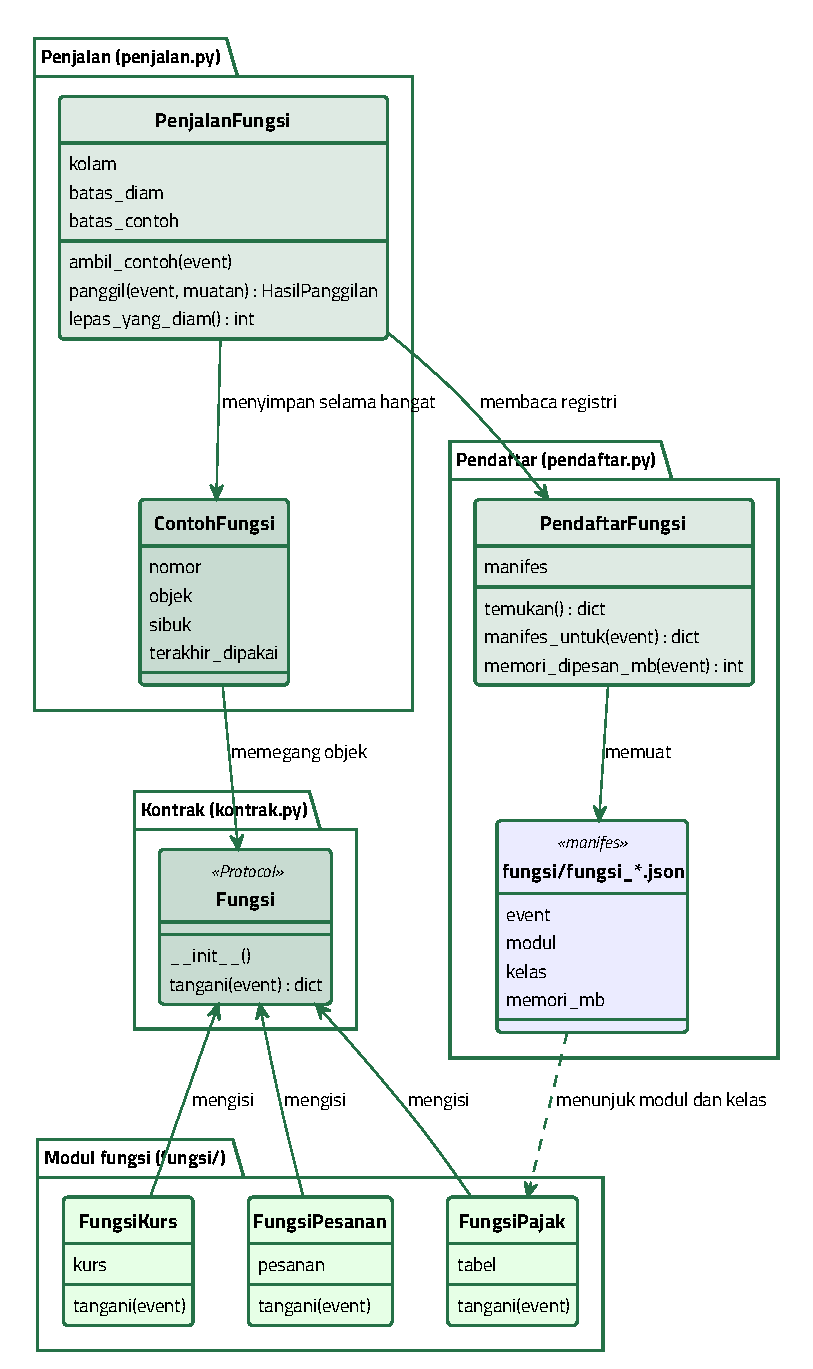
\includegraphics[width=\textwidth, height=0.76\textheight,
      keepaspectratio]{kelas-serverless.pdf}
  \end{center}
\end{frame}

\begin{frame}{{\Large Penjelasan \textit{Class Diagram}}}
  \vspace{10pt}
  \begin{itemize}\small
    \item Tidak ada panah dari penjalan menuju ketiga fungsi, sedangkan panah
          dari registri menuju manifes justru ada.
    \item Nama kelas setiap fungsi tertulis di dalam manifesnya, bukan di dalam
          kode penjalan.
    \item Ketiga fungsi memenuhi kontrak yang sama, yaitu konstruktor tanpa
          argumen ditambah metode \texttt{tangani}.
    \item Harganya, kesalahan ketik nama kelas tidak lagi tertangkap saat
          impor, melainkan saat event pertamanya datang.
  \end{itemize}

  \vspace{10pt}
  {\small Pertukarannya sama seperti pada Bab 5, yaitu kelenturan ditebus
  dengan pemeriksaan yang bergeser ke waktu jalan.}
\end{frame}

\begin{frame}{{\Large \textit{Summary}}}
  \vspace{10pt}
  \begin{itemize}\small
    \item Fungsi hanya dimuat ketika \textit{event}-nya datang, lalu dilepas sesudah diam
          melewati batas.
    \item Pemuatan yang ditunda dibayar di muka, yaitu \textit{cold start}
          fungsi pajak 120,5837 ms melawan 0,0059 ms pada \textit{warm start}.
    \item Yang dibeli terbaca saat diam, yaitu 16,0 KiB melawan 21.179,3 KiB,
          dan 20,88 melawan 1.800,00 gigabita detik per jam.
    \item Lonjakan yang menimpa kolam kosong membuat delapan dari dua belas
          \textit{request} menunggu, dengan median 696,9689 ms.
  \end{itemize}

  \vspace{10pt}
  {\small Pesan utamanya, tanpa server memindahkan biaya dari waktu diam ke
  waktu mulai. Pemindahan itu menguntungkan selama \textit{request}-nya jarang.}
\end{frame}

\begin{frame}[fragile]{{\Large Persiapan Latihan}}
  \vspace{5pt}
\begin{lstlisting}[language=bash]
bash sources/siapkan_venv.sh
source .venv/bin/activate
cd sources/chapter14
python penjalan.py
# Panggilan 1 dingin=True Init 130.342 ms  tangani 0.023 ms  total 130.375 ms
# Panggilan 2 dingin=False Init 0.000 ms  tangani 0.017 ms  total 0.032 ms
# Contoh dilepas seluruhnya: 1
\end{lstlisting}

  \vspace{6pt}
  {\small Bab ini hanya memakai pustaka standar Python. Langkah lengkap, tabel
  contoh, dan lembar isian ada di modul Bab 14, yang menjadi rujukan utama
  latihan ini.}
\end{frame}

\begin{frame}[fragile]{{\Large Latihan 1: \textit{Cold Start Cost}}}
  \vspace{2pt}
  {\small Tujuan: menguji klaim bahwa \textit{cold start} hanya persoalan kecil.}

  \vspace{2pt}
\begin{lstlisting}[language=bash]
python ukur_mulai.py
# Median cold start            : 120.5837 ms
# Median warm start            : 0.0059 ms
# Range dibagi selisih         : 0.0004 kali
\end{lstlisting}

  \vspace{2pt}
  \begin{enumerate}\small
    \item Catat kedelapan angka latensi kedua fungsi.
    \item Tunjukkan baris pada \texttt{fungsi\_pajak.py} yang membuat fase
          \texttt{Init} menjadi berat.
    \item Ubah \texttt{LANGKAH\_TABEL} dari 1.000 menjadi 100, lalu catat
          perubahan median \textit{cold start}.
  \end{enumerate}

  \vspace{2pt}
  {\small Pertanyaan: mengapa median \textit{warm start} kedua fungsi belum
  dapat dibedakan?}
\end{frame}

\begin{frame}[fragile]{{\Large Latihan 2: \textit{Idle Cost}}}
  \vspace{2pt}
  {\small Tujuan: mengukur harga yang dibayar ketika \textit{request}-nya tidak
  datang.}

  \vspace{2pt}
\begin{lstlisting}[language=bash]
python ukur_sumber_daya.py
# Memori penjalan saat nol      : 16.0 KiB
# Memori layanan saat menganggur: 21179.3 KiB
# Titik impas bila cold start   : 62,069 request per jam
\end{lstlisting}

  \vspace{2pt}
  \begin{enumerate}\small
    \item Catat kelima baris keadaan diam beserta ketiga baris gigabita detik.
    \item Ubah \texttt{memori\_mb} pada manifes pajak dari 256 menjadi 512,
          lalu catat perubahan titik impasnya.
    \item Hitung sendiri titik impasnya, lalu bandingkan dengan baris yang
          dicetak skrip.
  \end{enumerate}

  \vspace{2pt}
  {\small Pertanyaan: pada kerapatan \textit{request} seperti apa layanan hidup
  justru lebih murah?}
\end{frame}

\begin{frame}[fragile]{{\Large Latihan 3: \textit{Concurrency Limit}}}
  \vspace{2pt}
  {\small Tujuan: membuktikan biaya terbesar muncul pada lonjakan ke kolam
  kosong.}

  \vspace{2pt}
\begin{lstlisting}[language=bash]
python ukur_lonjakan.py
# Request menunggu           : 80
# Median latensi                : 696.9689 ms
# Median latensi, kolam hangat  : 0.0127 ms
\end{lstlisting}

  \vspace{2pt}
  \begin{enumerate}\small
    \item Catat kelima baris hasil ketiga keadaannya.
    \item Naikkan \texttt{BATAS\_CONTOH} dari 4 menjadi 12, lalu catat
          perubahan \textit{request} yang menunggu.
    \item Kembalikan batasnya, lalu naikkan \texttt{JUMLAH\_SERENTAK} dari 12
          menjadi 24 dan catat median latensinya.
  \end{enumerate}

  \vspace{2pt}
  {\small Pertanyaan: kapan susunan tanpa server layak dipilih untuk layanan
  kampus yang \textit{request}-nya menumpuk?}
\end{frame}

\end{document}
